% Options for packages loaded elsewhere
\PassOptionsToPackage{unicode}{hyperref}
\PassOptionsToPackage{hyphens}{url}
\PassOptionsToPackage{dvipsnames,svgnames,x11names}{xcolor}
%
\documentclass[
  10pt,
]{article}
\usepackage{amsmath,amssymb}
\usepackage{iftex}
\ifPDFTeX
  \usepackage[T1]{fontenc}
  \usepackage[utf8]{inputenc}
  \usepackage{textcomp} % provide euro and other symbols
\else % if luatex or xetex
  \usepackage{unicode-math} % this also loads fontspec
  \defaultfontfeatures{Scale=MatchLowercase}
  \defaultfontfeatures[\rmfamily]{Ligatures=TeX,Scale=1}
\fi
\usepackage{lmodern}
\ifPDFTeX\else
  % xetex/luatex font selection
\fi
% Use upquote if available, for straight quotes in verbatim environments
\IfFileExists{upquote.sty}{\usepackage{upquote}}{}
\IfFileExists{microtype.sty}{% use microtype if available
  \usepackage[]{microtype}
  \UseMicrotypeSet[protrusion]{basicmath} % disable protrusion for tt fonts
}{}
\makeatletter
\@ifundefined{KOMAClassName}{% if non-KOMA class
  \IfFileExists{parskip.sty}{%
    \usepackage{parskip}
  }{% else
    \setlength{\parindent}{0pt}
    \setlength{\parskip}{6pt plus 2pt minus 1pt}}
}{% if KOMA class
  \KOMAoptions{parskip=half}}
\makeatother
\usepackage{xcolor}
\usepackage[left=2cm, right=2cm, top=2cm, bottom=3cm, footskip = .5cm]{geometry}
\usepackage{longtable,booktabs,array}
\usepackage{calc} % for calculating minipage widths
% Correct order of tables after \paragraph or \subparagraph
\usepackage{etoolbox}
\makeatletter
\patchcmd\longtable{\par}{\if@noskipsec\mbox{}\fi\par}{}{}
\makeatother
% Allow footnotes in longtable head/foot
\IfFileExists{footnotehyper.sty}{\usepackage{footnotehyper}}{\usepackage{footnote}}
\makesavenoteenv{longtable}
\usepackage{graphicx}
\makeatletter
\def\maxwidth{\ifdim\Gin@nat@width>\linewidth\linewidth\else\Gin@nat@width\fi}
\def\maxheight{\ifdim\Gin@nat@height>\textheight\textheight\else\Gin@nat@height\fi}
\makeatother
% Scale images if necessary, so that they will not overflow the page
% margins by default, and it is still possible to overwrite the defaults
% using explicit options in \includegraphics[width, height, ...]{}
\setkeys{Gin}{width=\maxwidth,height=\maxheight,keepaspectratio}
% Set default figure placement to htbp
\makeatletter
\def\fps@figure{htbp}
\makeatother
\setlength{\emergencystretch}{3em} % prevent overfull lines
\providecommand{\tightlist}{%
  \setlength{\itemsep}{0pt}\setlength{\parskip}{0pt}}
\setcounter{secnumdepth}{-\maxdimen} % remove section numbering
% Set up the fonts
\usepackage[urw-palatino]{mathdesign}
\usepackage[T1]{fontenc}

% Add accessibility support from http://www.richschwinn.com/accessibility
\RequirePackage{accsupp}
\RequirePackage{pdfcomment}
\newcommand{\AccTool}[2]{\BeginAccSupp{method=pdfstringdef,unicode,Alt={{#1}}}\pdftooltip{{#2}}{{#1}}\EndAccSupp{}}

% Set the language for 508
\hypersetup{
  pdftitle = {title},
  pdflang = en-US}


% Set up the headers and footers
\usepackage{graphicx}
\usepackage{fancyhdr}
\usepackage{ifthen}
%\usepackage{everypage-1x}
\usepackage{float}
%\usepackage{subfig}
%\usepackage{subcaption}

% Avoid struggling over figure and table float in Rmarkdown
\let\origfigure\figure
\let\endorigfigure\endfigure
\renewenvironment{figure}[1][2] {
    \expandafter\origfigure\expandafter[H]
} {
    \endorigfigure
}

\let\origtable\table
\let\endorigtable\endtable
\renewenvironment{table}[1][2] {
    \expandafter\origtable\expandafter[H]
} {
    \endorigtable
}

% First page has the large title and NOAA logo
\pagestyle{fancy}
\fancyhf{}
\setlength\headheight{40pt}
\fancyheadoffset[L]{0.5cm}
\cfoot{\thepage}

\fancyheadinit{%
   \ifthenelse{\value{page}=4}%
      {\fancyhead[R]{
\includegraphics[width=40pt]{images/NOAA_logo.png} \\ \textsf{\emph{March 24, 2025}}}
       \fancyhead[L]{\textsf{\LARGE State of the Ecosystem 2025: Mid-Atlantic}}
      }%
      {\fancyhead[R]{}
       \fancyhead[L]{\textsf{\emph{State of the Ecosystem 2025: Mid-Atlantic}}}
      }
}



\renewcommand{\headrulewidth}{0.4pt}
\renewcommand{\footrulewidth}{0pt}

% Make caption fonts a bit smaller
\usepackage[font={small}]{caption}


% Change section labels to san serif
\usepackage{sectsty}
\allsectionsfont{\normalfont\sffamily\bfseries}
\usepackage{multirow}
\usepackage{multicol}
\usepackage{colortbl}
\usepackage{hhline}
\newlength\Oldarrayrulewidth
\newlength\Oldtabcolsep
\usepackage{longtable}
\usepackage{array}
\usepackage{hyperref}
\usepackage{float}
\usepackage{wrapfig}
\ifLuaTeX
  \usepackage{selnolig}  % disable illegal ligatures
\fi
\usepackage{bookmark}
\IfFileExists{xurl.sty}{\usepackage{xurl}}{} % add URL line breaks if available
\urlstyle{same}
\hypersetup{
  colorlinks=true,
  linkcolor={Maroon},
  filecolor={Maroon},
  citecolor={Blue},
  urlcolor={blue},
  pdfcreator={LaTeX via pandoc}}

\author{}
\date{\vspace{-2.5em}}

\begin{document}

\setcounter{page}{4}
\thispagestyle{fancy}

\section{Introduction}\label{introduction}

\subsection{About This Report}\label{about-this-report}

This report is for the Mid-Atlantic Fishery Management Council (MAFMC). The purpose of this report is to synthesize ecosystem information to allow the MAFMC to better meet fishery management objectives, and to update the MAFMC's Ecosystem Approach to Fishery Management (EAFM) risk assessment. The major messages of the report are synthesized on pages 1 and 2, with highlights of 2024 ecosystem events on page 3.

The information in this report is organized into two main sections; \hyperref[performance-relative-to-fishery-management-objectives]{performance measured against ecosystem-level management objectives} (Table \ref{tab:management-objectives}), and potential \hyperref[risks-to-meeting-fishery-management-objectives]{risks to meeting fishery management objectives} (Table \ref{tab:management-risks}: \hyperref[climate-and-ecosystem-change]{climate change} and \hyperref[other-ocean-uses-offshore-wind]{other ocean uses}). A final section highlights \hyperref[highlights]{notable 2024 ecosystem observations}.

\subsection{Report structure}\label{report-structure}

A glossary of terms\footnote{\url{https://noaa-edab.github.io/tech-doc/glossary.html}}, detailed technical methods documentation\footnote{\url{https://noaa-edab.github.io/tech-doc/}}, indicator data\footnote{\url{https://noaa-edab.github.io/ecodata/}}, and detailed indicator descriptions\footnote{\url{https://noaa-edab.github.io/catalog/index.html}} are available online. We recommend new readers first review the details of standard figure formatting (Fig. \ref{fig:docformat}a), categorization of fish and invertebrate species into feeding guilds (Table \ref{tab:species-groupings}), and definitions of ecological production units (EPUs, including the Mid-Atlantic Bight, MAB; Fig. \ref{fig:docformat}b) provided at the end of the document.

The two main sections contain subsections for each management objective or potential risk. Within each subsection, we first review observed trends for indicators representing each objective or risk, including the status of the most recent data year relative to a threshold (if available) or relative to the long-term average. Second, we identify potential drivers of observed trends, and synthesize results of indicators related to those drivers to outline potential implications for management. For example, if there are multiple drivers related to an indicator trend, do indicators associated with the drivers have similar trends, and can any drivers be affected by management action(s)? We emphasize that these implications are intended to represent testable hypotheses at present, rather than ``answers,'' because the science behind these indicators and syntheses continues to develop.

\global\setlength{\Oldarrayrulewidth}{\arrayrulewidth}

\global\setlength{\Oldtabcolsep}{\tabcolsep}

\setlength{\tabcolsep}{2pt}

\renewcommand*{\arraystretch}{1}



\providecommand{\ascline}[3]{\noalign{\global\arrayrulewidth #1}\arrayrulecolor[HTML]{#2}\cline{#3}}

\begin{longtable}[c]{|p{1.77in}|p{4.09in}}

\caption{Ecosystem-scale\ fishery\ management\ objectives\ in\ the\ Mid-Atlantic\ Bight}\label{tab:management-objectives}\\

\ascline{1.5pt}{666666}{1-2}

\multicolumn{1}{>{\raggedright}m{\dimexpr 1.77in+0\tabcolsep}}{\textcolor[HTML]{000000}{\fontsize{9}{9}\selectfont{Objective\ categories}}} & \multicolumn{1}{>{\raggedright}m{\dimexpr 4.09in+0\tabcolsep}}{\textcolor[HTML]{000000}{\fontsize{9}{9}\selectfont{Indicators\ reported}}} \\

\ascline{1.5pt}{666666}{1-2}\endfirsthead \caption[]{Ecosystem-scale\ fishery\ management\ objectives\ in\ the\ Mid-Atlantic\ Bight}\label{tab:management-objectives}\\

\ascline{1.5pt}{666666}{1-2}

\multicolumn{1}{>{\raggedright}m{\dimexpr 1.77in+0\tabcolsep}}{\textcolor[HTML]{000000}{\fontsize{9}{9}\selectfont{Objective\ categories}}} & \multicolumn{1}{>{\raggedright}m{\dimexpr 4.09in+0\tabcolsep}}{\textcolor[HTML]{000000}{\fontsize{9}{9}\selectfont{Indicators\ reported}}} \\

\ascline{1.5pt}{666666}{1-2}\endhead



\multicolumn{2}{>{\raggedright}m{\dimexpr 5.86in+2\tabcolsep}}{\textcolor[HTML]{000000}{\fontsize{9}{9}\selectfont{\textbf{Objectives:\ Provisioning\ and\ Cultural\ Services}}}} \\





\multicolumn{1}{>{\raggedright}m{\dimexpr 1.77in+0\tabcolsep}}{\textcolor[HTML]{000000}{\fontsize{9}{9}\selectfont{Seafood\ Production}}} & \multicolumn{1}{>{\raggedright}m{\dimexpr 4.09in+0\tabcolsep}}{\textcolor[HTML]{000000}{\fontsize{9}{9}\selectfont{Landings;\ commercial\ total\ and\ by\ feeding\ guild;\ recreational\ harvest}}} \\





\multicolumn{1}{>{\raggedright}m{\dimexpr 1.77in+0\tabcolsep}}{\textcolor[HTML]{000000}{\fontsize{9}{9}\selectfont{Commercial\ Profits}}} & \multicolumn{1}{>{\raggedright}m{\dimexpr 4.09in+0\tabcolsep}}{\textcolor[HTML]{000000}{\fontsize{9}{9}\selectfont{Revenue\ decomposed\ to\ price\ and\ volume}}} \\





\multicolumn{1}{>{\raggedright}m{\dimexpr 1.77in+0\tabcolsep}}{\textcolor[HTML]{000000}{\fontsize{9}{9}\selectfont{Recreational\ Opportunities}}} & \multicolumn{1}{>{\raggedright}m{\dimexpr 4.09in+0\tabcolsep}}{\textcolor[HTML]{000000}{\fontsize{9}{9}\selectfont{Angler\ trips;\ recreational\ fleet\ diversity}}} \\





\multicolumn{1}{>{\raggedright}m{\dimexpr 1.77in+0\tabcolsep}}{\textcolor[HTML]{000000}{\fontsize{9}{9}\selectfont{Stability}}} & \multicolumn{1}{>{\raggedright}m{\dimexpr 4.09in+0\tabcolsep}}{\textcolor[HTML]{000000}{\fontsize{9}{9}\selectfont{Diversity\ indices\ (fishery\ and\ ecosystem)}}} \\





\multicolumn{1}{>{\raggedright}m{\dimexpr 1.77in+0\tabcolsep}}{\textcolor[HTML]{000000}{\fontsize{9}{9}\selectfont{Social\ \&\ Cultural}}} & \multicolumn{1}{>{\raggedright}m{\dimexpr 4.09in+0\tabcolsep}}{\textcolor[HTML]{000000}{\fontsize{9}{9}\selectfont{Community\ fishing\ engagement\ and\ social\ vulnerability\ status}}} \\





\multicolumn{1}{>{\raggedright}m{\dimexpr 1.77in+0\tabcolsep}}{\textcolor[HTML]{000000}{\fontsize{9}{9}\selectfont{Protected\ Species}}} & \multicolumn{1}{>{\raggedright}m{\dimexpr 4.09in+0\tabcolsep}}{\textcolor[HTML]{000000}{\fontsize{9}{9}\selectfont{Bycatch;\ population\ (adult\ and\ juvenile)\ numbers;\ mortalities}}} \\





\multicolumn{2}{>{\raggedright}m{\dimexpr 5.86in+2\tabcolsep}}{\textcolor[HTML]{000000}{\fontsize{9}{9}\selectfont{\textbf{Potential\ Drivers:\ Supporting\ and\ Regulating\ Services}}}} \\





\multicolumn{1}{>{\raggedright}m{\dimexpr 1.77in+0\tabcolsep}}{\textcolor[HTML]{000000}{\fontsize{9}{9}\selectfont{Management}}} & \multicolumn{1}{>{\raggedright}m{\dimexpr 4.09in+0\tabcolsep}}{\textcolor[HTML]{000000}{\fontsize{9}{9}\selectfont{Stock\ status;\ catch\ compared\ with\ catch\ limits}}} \\





\multicolumn{1}{>{\raggedright}m{\dimexpr 1.77in+0\tabcolsep}}{\textcolor[HTML]{000000}{\fontsize{9}{9}\selectfont{Biomass}}} & \multicolumn{1}{>{\raggedright}m{\dimexpr 4.09in+0\tabcolsep}}{\textcolor[HTML]{000000}{\fontsize{9}{9}\selectfont{Biomass\ or\ abundance\ by\ feeding\ guild\ from\ surveys}}} \\





\multicolumn{1}{>{\raggedright}m{\dimexpr 1.77in+0\tabcolsep}}{\textcolor[HTML]{000000}{\fontsize{9}{9}\selectfont{Environment}}} & \multicolumn{1}{>{\raggedright}m{\dimexpr 4.09in+0\tabcolsep}}{\textcolor[HTML]{000000}{\fontsize{9}{9}\selectfont{Climate\ and\ ecosystem\ risk\ indicators\ listed\ in\ Table\ 2}}} \\

\ascline{1.5pt}{666666}{1-2}



\end{longtable}



\arrayrulecolor[HTML]{000000}

\global\setlength{\arrayrulewidth}{\Oldarrayrulewidth}

\global\setlength{\tabcolsep}{\Oldtabcolsep}

\renewcommand*{\arraystretch}{1}

\newpage

\global\setlength{\Oldarrayrulewidth}{\arrayrulewidth}

\global\setlength{\Oldtabcolsep}{\tabcolsep}

\setlength{\tabcolsep}{2pt}

\renewcommand*{\arraystretch}{1}



\providecommand{\ascline}[3]{\noalign{\global\arrayrulewidth #1}\arrayrulecolor[HTML]{#2}\cline{#3}}

\begin{longtable}[c]{|p{1.00in}|p{2.20in}|p{2.80in}}

\caption{Risks\ to\ meeting\ fishery\ management\ objectives\ in\ the\ Mid-Atlantic\ Bight}\label{tab:management-risks}\\

\ascline{1.5pt}{666666}{1-3}

\multicolumn{1}{>{\raggedright}m{\dimexpr 1in+0\tabcolsep}}{\textcolor[HTML]{000000}{\fontsize{9}{9}\selectfont{Risk\ categories}}} & \multicolumn{1}{>{\raggedright}m{\dimexpr 2.2in+0\tabcolsep}}{\textcolor[HTML]{000000}{\fontsize{9}{9}\selectfont{Observation\ indicators\ reported}}} & \multicolumn{1}{>{\raggedright}m{\dimexpr 2.8in+0\tabcolsep}}{\textcolor[HTML]{000000}{\fontsize{9}{9}\selectfont{Potential\ driver\ indicators\ reported}}} \\

\ascline{1.5pt}{666666}{1-3}\endfirsthead \caption[]{Risks\ to\ meeting\ fishery\ management\ objectives\ in\ the\ Mid-Atlantic\ Bight}\label{tab:management-risks}\\

\ascline{1.5pt}{666666}{1-3}

\multicolumn{1}{>{\raggedright}m{\dimexpr 1in+0\tabcolsep}}{\textcolor[HTML]{000000}{\fontsize{9}{9}\selectfont{Risk\ categories}}} & \multicolumn{1}{>{\raggedright}m{\dimexpr 2.2in+0\tabcolsep}}{\textcolor[HTML]{000000}{\fontsize{9}{9}\selectfont{Observation\ indicators\ reported}}} & \multicolumn{1}{>{\raggedright}m{\dimexpr 2.8in+0\tabcolsep}}{\textcolor[HTML]{000000}{\fontsize{9}{9}\selectfont{Potential\ driver\ indicators\ reported}}} \\

\ascline{1.5pt}{666666}{1-3}\endhead



\multicolumn{3}{>{\raggedright}m{\dimexpr 6in+4\tabcolsep}}{\textcolor[HTML]{000000}{\fontsize{9}{9}\selectfont{\textbf{Climate\ and\ Ecosystem\ Risks}}}} \\





\multicolumn{1}{>{\raggedright}m{\dimexpr 1in+0\tabcolsep}}{\textcolor[HTML]{000000}{\fontsize{9}{9}\selectfont{Risks\ to\ Managing\ Spatially}}} & \multicolumn{1}{>{\raggedright}m{\dimexpr 2.2in+0\tabcolsep}}{\textcolor[HTML]{000000}{\fontsize{9}{9}\selectfont{Managed\ species\ (fish\ and\ cetacean)\ distribution\ shifts}}} & \multicolumn{1}{>{\raggedright}m{\dimexpr 2.8in+0\tabcolsep}}{\textcolor[HTML]{000000}{\fontsize{9}{9}\selectfont{Benthic\ and\ pelagic\ forage\ distribution;\ ocean\ temperature,\ changes\ in\ currents\ and\ cold\ pool}}} \\





\multicolumn{1}{>{\raggedright}m{\dimexpr 1in+0\tabcolsep}}{\textcolor[HTML]{000000}{\fontsize{9}{9}\selectfont{Risks\ to\ Managing\ Seasonally}}} & \multicolumn{1}{>{\raggedright}m{\dimexpr 2.2in+0\tabcolsep}}{\textcolor[HTML]{000000}{\fontsize{9}{9}\selectfont{Managed\ species\ spawning\ and\ migration\ timing\ changes}}} & \multicolumn{1}{>{\raggedright}m{\dimexpr 2.8in+0\tabcolsep}}{\textcolor[HTML]{000000}{\fontsize{9}{9}\selectfont{Habitat\ timing:\ Length\ of\ ocean\ summer,\ cold\ pool\ seasonal\ persistence}}} \\





\multicolumn{1}{>{\raggedright}m{\dimexpr 1in+0\tabcolsep}}{\textcolor[HTML]{000000}{\fontsize{9}{9}\selectfont{Risks\ to\ Setting\ Catch\ Limits}}} & \multicolumn{1}{>{\raggedright}m{\dimexpr 2.2in+0\tabcolsep}}{\textcolor[HTML]{000000}{\fontsize{9}{9}\selectfont{Managed\ species\ body\ condition\ and\ recruitment\ changes}}} & \multicolumn{1}{>{\raggedright}m{\dimexpr 2.8in+0\tabcolsep}}{\textcolor[HTML]{000000}{\fontsize{9}{9}\selectfont{Benthic\ and\ pelagic\ forage\ quality\ \&\ abundance:\ ocean\ temperature\ \&\ acidification\ }}} \\





\multicolumn{3}{>{\raggedright}m{\dimexpr 6in+4\tabcolsep}}{\textcolor[HTML]{000000}{\fontsize{9}{9}\selectfont{\textbf{Other\ Ocean\ Uses\ Risks}}}} \\





\multicolumn{1}{>{\raggedright}m{\dimexpr 1in+0\tabcolsep}}{\textcolor[HTML]{000000}{\fontsize{9}{9}\selectfont{Offshore\ Wind\ Risks}}} & \multicolumn{1}{>{\raggedright}m{\dimexpr 2.2in+0\tabcolsep}}{\textcolor[HTML]{000000}{\fontsize{9}{9}\selectfont{Fishery\ revenue\ and\ landings\ from\ wind\ lease\ areas\ by\ species\ and\ port}}} & \multicolumn{1}{>{\raggedright}m{\dimexpr 2.8in+0\tabcolsep}}{\textcolor[HTML]{000000}{\fontsize{9}{9}\selectfont{Wind\ development\ speed;\ Protected\ species\ presence\ and\ \ hotspots}}} \\

\ascline{1.5pt}{666666}{1-3}



\end{longtable}



\arrayrulecolor[HTML]{000000}

\global\setlength{\arrayrulewidth}{\Oldarrayrulewidth}

\global\setlength{\tabcolsep}{\Oldtabcolsep}

\renewcommand*{\arraystretch}{1}

\section{Performance Relative to Fishery Management Objectives}\label{performance-relative-to-fishery-management-objectives}

In this section, we examine indicators related to broad, ecosystem-level fishery management objectives. We also provide hypotheses on the implications of these trends---why we are seeing them, what's driving them, and potential or observed regime shifts or changes in ecosystem structure. Identifying multiple drivers, regime shifts, and potential changes to ecosystem structure, as well as identifying the most vulnerable resources, can help managers determine whether anything needs to be done differently to meet objectives and how to prioritize upcoming issues/risks.

\subsection{Seafood Production}\label{seafood-production}

\subsubsection{Indicators: Landings; commercial and recreational}\label{indicators-landings-commercial-and-recreational}

This year, we present updated indicators for total \href{https://noaa-edab.github.io/catalog/comdat.html}{commercial landings}, (includes seafood, bait, and industrial landings), U.S. seafood landings, and Council-managed U.S. seafood landings. Total commercial landings within the Mid-Atlantic have declined over the long term, and both total U.S. and Mid-Atlantic managed seafood landings are near their all time low (Fig. \ref{fig:total-landings}).

\begin{figure}

{\centering 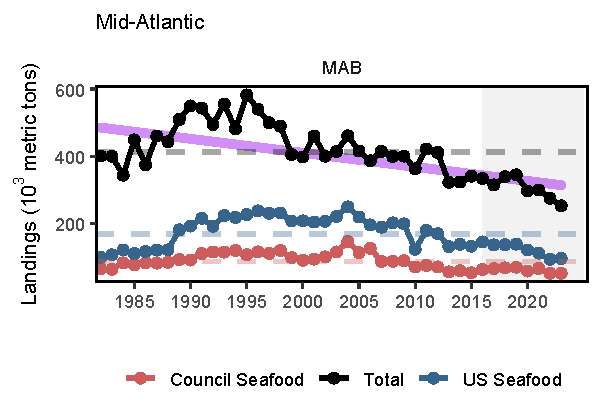
\includegraphics{C:/Users/abigail.tyrell/Documents/code/READ-EDAB-SOE_reports/midatlantic_files/figure-latex/total-landings-1} 

}

\caption{Total commercial landings (black), total U.S. seafood landings (blue), and Mid-Atlantic managed U.S. seafood landings (red), with significant decline (purple) in total landings.}\label{fig:total-landings}
\end{figure}

Commercial landings by guild include all species and all uses, and are reported as total for the guild and the MAFMC managed species within the \href{https://noaa-edab.github.io/catalog/species_groupings.html}{guild}. Landings of benthos have been below the long term average since 2010, primarily driven by surf clam and ocean quahog, with scallops now contributing to the decline as well. Total landings of planktivores is presenting a significant downward trend, primarily due to decreases in species not managed by the MAFMC (Atlantic herring and Atlantic menhaden; Fig. \ref{fig:comm-landings}).

\begin{figure}

{\centering 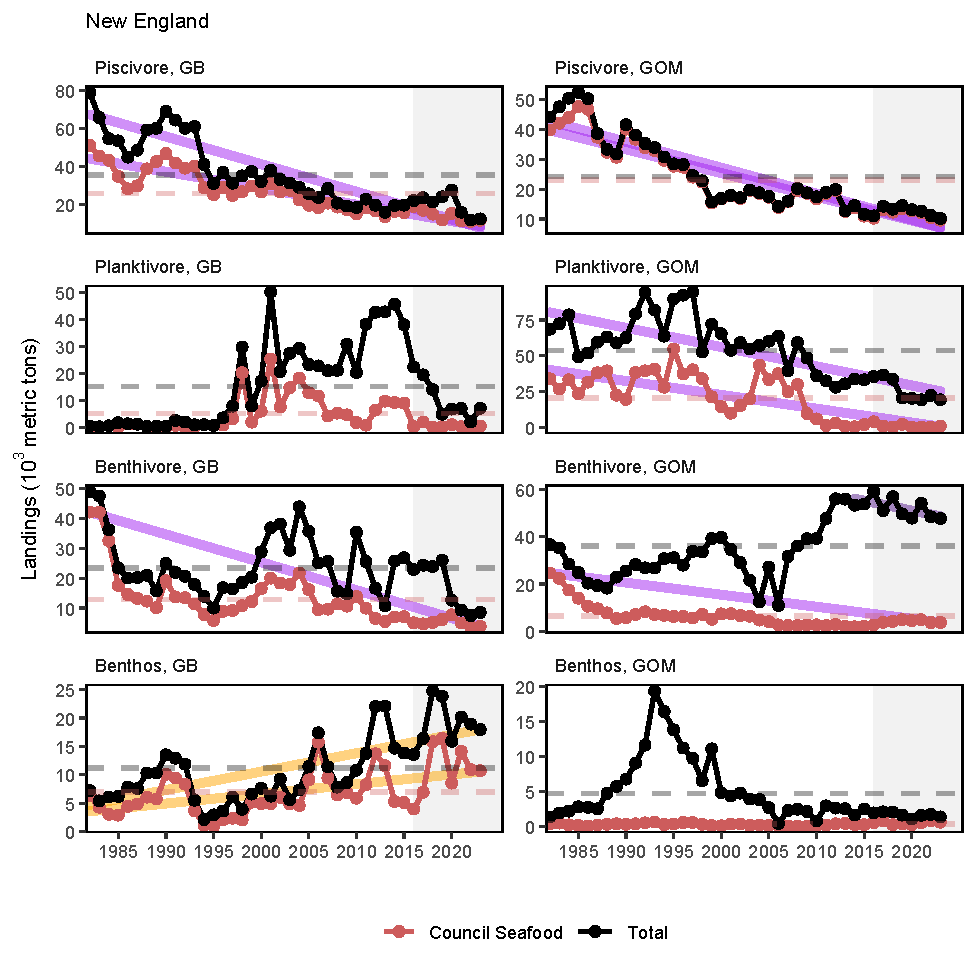
\includegraphics{C:/Users/abigail.tyrell/Documents/code/READ-EDAB-SOE_reports/midatlantic_files/figure-latex/comm-landings-1} 

}

\caption{Total commercial landings in the Mid-Atlantic Bight (black) and MAFMC-managed U.S seafood landings (red) by feeding guild, with significant declines (purple) in total planktivore landings.}\label{fig:comm-landings}
\end{figure}

\href{https://noaa-edab.github.io/catalog/community_climate_vulnerability.html}{Community Climate Change Risk indicators} have been developed to evaluate port specific landings and revenue risk in terms of commercial species climate vulnerability. The total climate vulnerability is a measure of to what degree a region's landings (or revenue) is dependent on species sensitive to different climate and environmental change factors including temperature and acidification. For ports combined across Mid-Atlantic states, the total climate vulnerability of landings ranged between moderate and high with a long term increase from 2000-2021 (Fig. \ref{fig:climatevul-land}).

\begin{figure}

{\centering 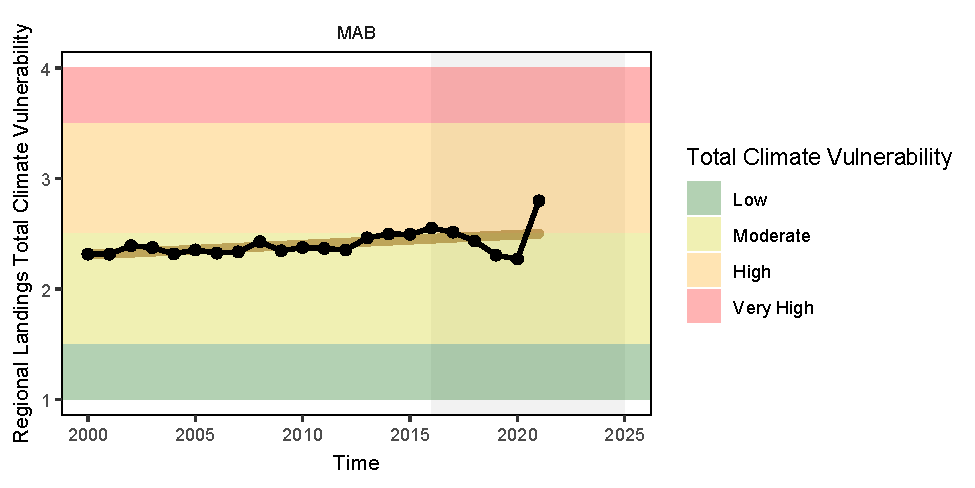
\includegraphics{C:/Users/abigail.tyrell/Documents/code/READ-EDAB-SOE_reports/midatlantic_files/figure-latex/climatevul-land-1} 

}

\caption{Mid-Atlantic region total climate vulnerability of commercial landings (sum of Mid-Atlantic port landings weighted by species climate vulnerability from Hare et al. 2016).}\label{fig:climatevul-land}
\end{figure}

\subsection{Commercial Profits}\label{commercial-profits}

\subsection{Recreational Opportunities}\label{recreational-opportunities}

\subsection{Stability}\label{stability}

\subsection{Community Social and Climate Vulnerability}\label{community-social-and-climate-vulnerability}

\subsection{Protected Species}\label{protected-species}

\section{Risks to Meeting Fishery Management Objectives}\label{risks-to-meeting-fishery-management-objectives}

\subsection{Climate and Ecosystem Change}\label{climate-and-ecosystem-change}

\subsection{Other Ocean Uses: Offshore Wind}\label{other-ocean-uses-offshore-wind}

\newpage

\subsubsection{2024 Highlights}\label{highlights}

This section intends to provide a record of \href{https://noaa-edab.github.io/catalog/observation_synthesis_2024.html}{noteworthy observations reported in 2024} across the Northeast U.S. region. The full ecosystem and fisheries impacts of many of these observations are still to be determined. They should, however, be noted and considered in future analyses and management decisions.

2024 global sea surface and air temperatures exceeded 2023 as the warmest year on record, but colder than average temperatures were observed in the Northeast U.S. Oceanographic and ecological conditions in the Northwest Atlantic were markedly different in 2024 compared to recent years.

\paragraph{Northwest Atlantic Phenomena}\label{northwest-atlantic-phenomena}

Late 2023 and early 2024 observations indicate movement of cooler and fresher water into the Northwest Atlantic, although there are seasonal and local exceptions to this pattern. Anomalously cold (Fig. \ref{fig:slopesea}) and low salinity conditions were recorded throughout the Northeast Shelf and were widespread across the Slope Sea for much of the year. These cooler and fresher conditions are linked to the southward movement of the eastern portion of the \href{https://noaa-edab.github.io/catalog/gsi.html}{Gulf Stream} and possibly an increased influx of Labrador Slope and Scotian Shelf water into the system.

\begin{figure}

{\centering 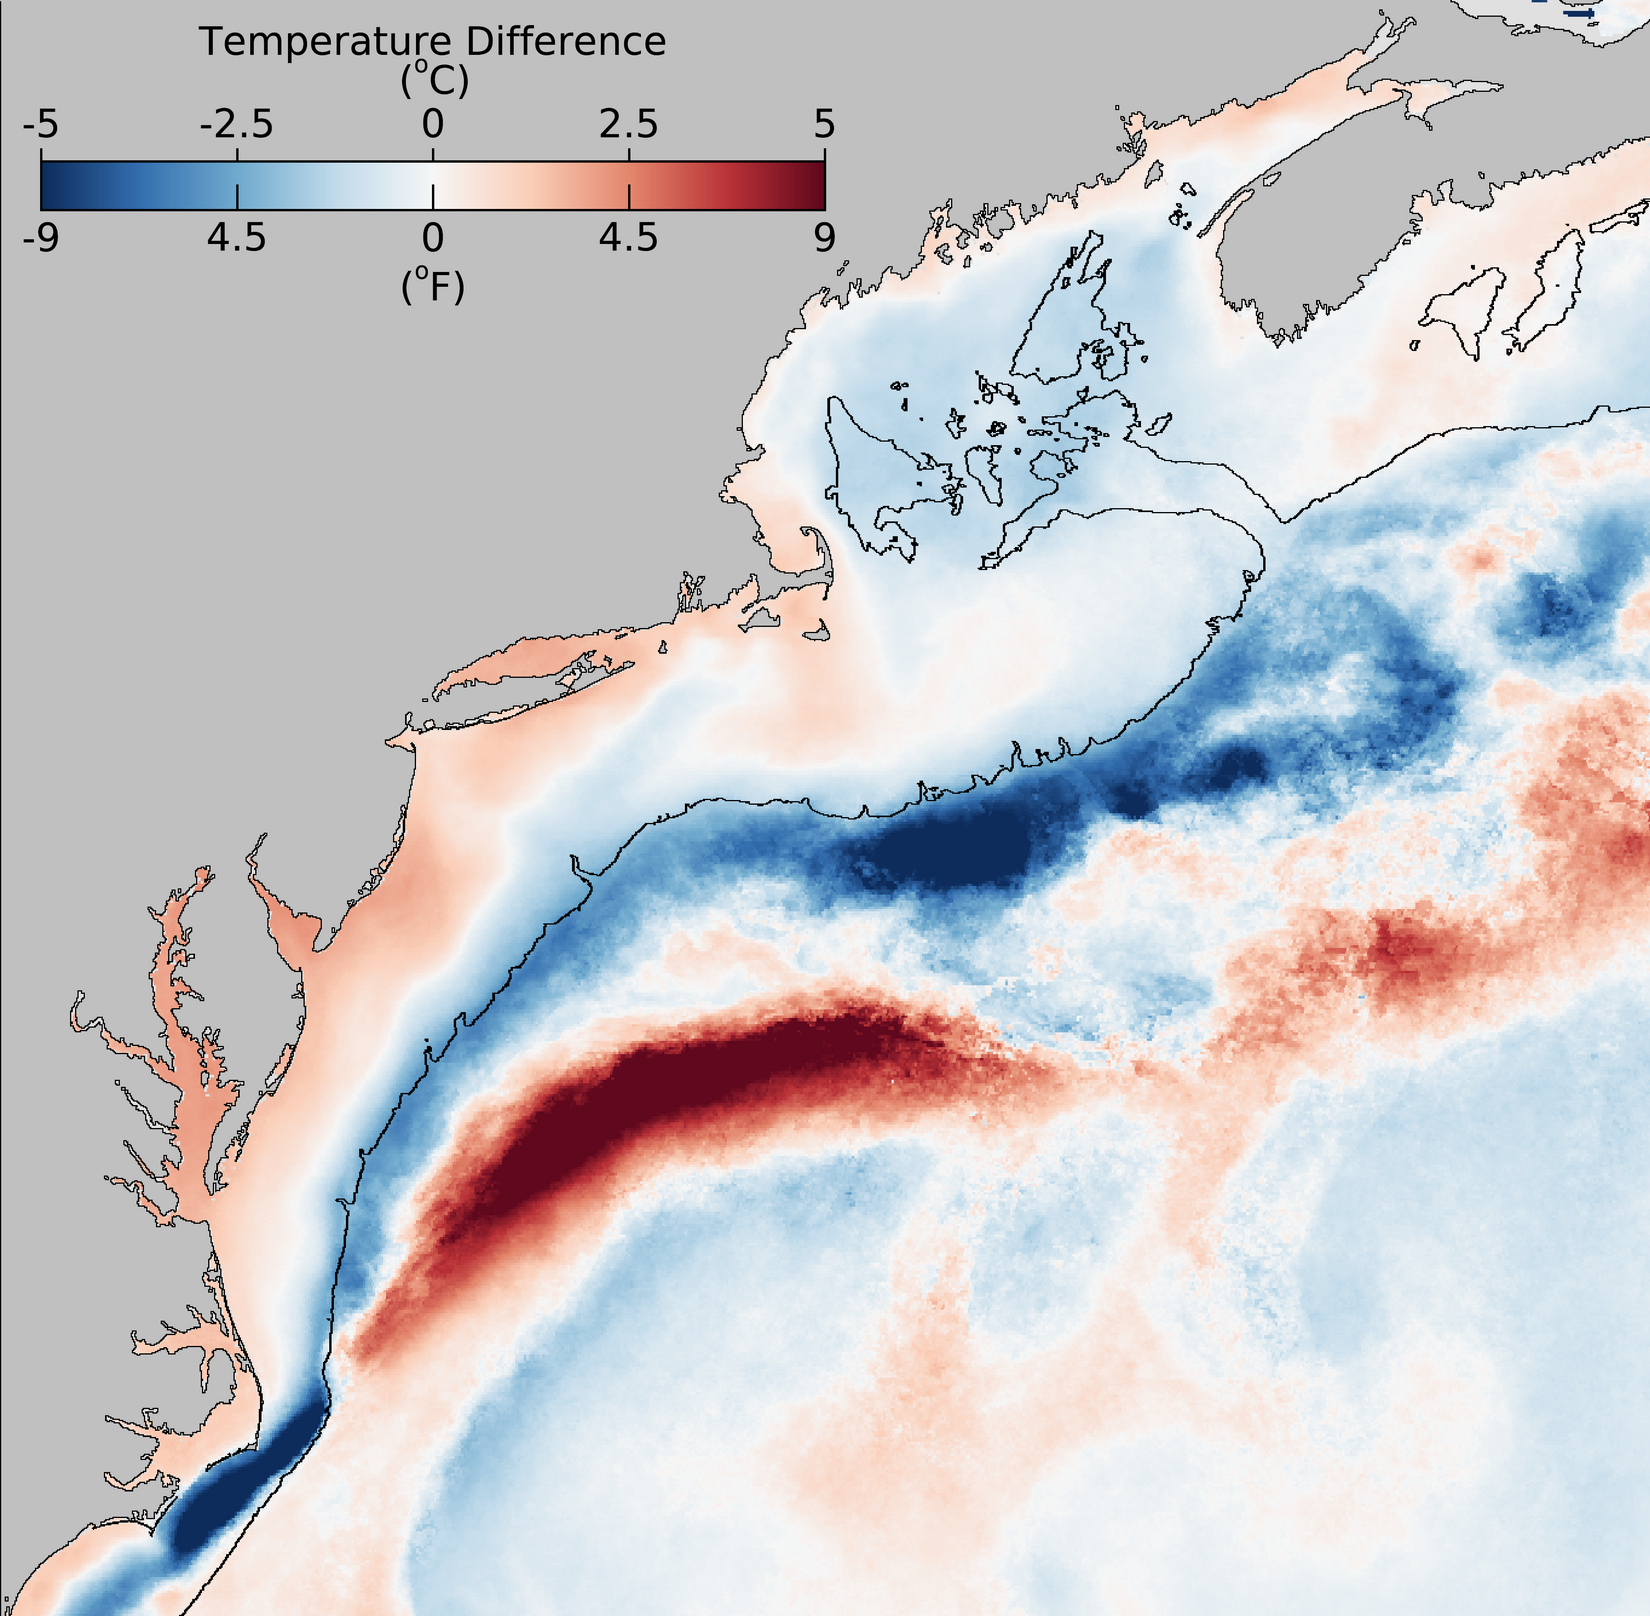
\includegraphics[width=0.65\linewidth]{midatlantic_files/figure-latex/slopesea-1} 

}

\caption{February 2024 sea surface temperature difference compared to the February 2000-2020 long-term mean from the NOAA Advanced Clear-Sky Processor for Ocean (ACSPO) Super-collated SST.}\label{fig:slopesea}
\end{figure}

In 2023, Labrador Slope water accounted for more than 50\% of the \href{https://noaa-edab.github.io/catalog/slopewater.html}{source water} entering the Gulf of Maine through the Northeast Channel (Fig. \ref{fig:slopewater}); data are still being processed for 2024. Colder, fresher water detected deep in the Jordan Basin for the \href{https://noaa-edab.github.io/catalog/observation_synthesis_2024.html}{first half of 2024} suggests an increased influx of Labrador Slope and Scotian Shelf water, which resulted in colder and fresher conditions throughout the Northwest Atlantic and contributed to the increased size and colder temperatures of the Mid-Atlantic \href{https://noaa-edab.github.io/catalog/cold_pool.html}{Cold Pool}.

\begin{figure}

{\centering 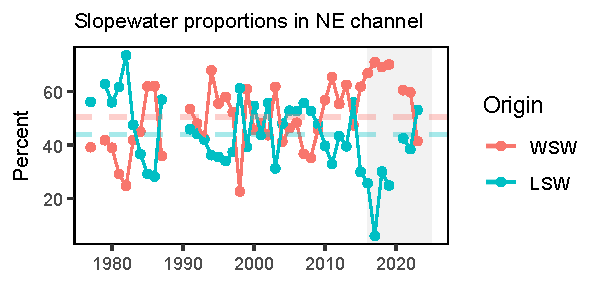
\includegraphics{C:/Users/abigail.tyrell/Documents/code/READ-EDAB-SOE_reports/midatlantic_files/figure-latex/slopewater-1} 

}

\caption{The proportion of Warm Slope Water (WSW) and Labrador Slope Water (LSW) enter the Gulf of Maine through the Northeast Channel. The orange and teal dashed lines represent the long-term proportion averages for the WSW and LSW respectively.}\label{fig:slopewater}
\end{figure}

\paragraph{Northeast Shelf and Local Phenomena}\label{northeast-shelf-and-local-phenomena}

The influx of the northern waters is likely linked to multiple observations across the Northeast Shelf including the uncommon presence of Arctic \emph{Calanus} zooplankton species in the Gulf of Maine, delayed migration of many species, and redistribution of some species. Several members of the fishing community noted delayed migration of species into typical fishing grounds. In particular, they attributed the delayed migration of longfin squid, black sea bass, and haddock to the cooler water temperatures. Many also reported redistribution of some species. Specifically, pollock, bluefin tuna, Atlantic mackerel, longfin squid, bluefish, and bonito were observed in surprising or unusual locations. Some species, such as Atlantic mackerel, were reported outside of typical fishing grounds and in higher abundance compared to recent years. Anglers also reported good catches of red drum in Chesapeake Bay and record high (since 1995) numbers were observed at Poplar Island survey location.

In the summer, Chesapeake Bay recorded warm temperatures and low bottom water dissolved oxygen that resulted in less than suitable habitat for species such as striped bass and blue crabs. These poor conditions can affect their distribution, growth, and survival. Additionally, lower than average spring and summer salinity negatively impacted oyster hatchery operations and increased the area of available habitat for invasive blue catfish, potentially increasing predation on blue crabs and other important finfish species.

During the summer months there were multiple prolonged upwelling events that brought cold water to the surface off the New Jersey coast. There was also an atypical phytoplankton bloom south of Long Island in late June to early July 2024, possibly linked to an upwelling event (Fig. \ref{fig:cocobloom}). The bloom was dominated by coccolithophores, which have an exoskeleton made up of calcium carbonate plates that can turn the water an opaque turquoise color. Large blooms of coccolithophores are unusual in this region, but they are not considered harmful and are grazed by zooplankton. Additionally, there were observations of multiple whale species aggregating near the Hudson Canyon between May and August.

\begin{figure}

{\centering 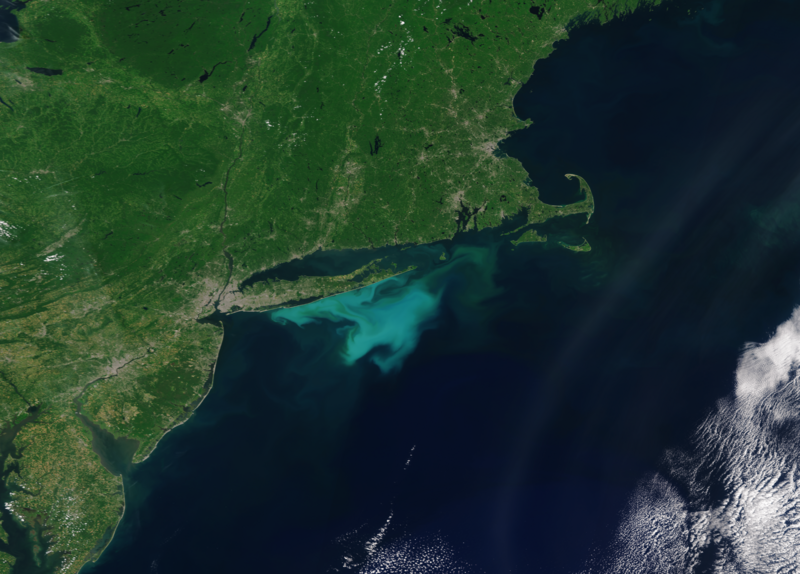
\includegraphics[width=0.55\linewidth]{midatlantic_files/figure-latex/cocobloom-1} 

}

\caption{An OLCI Sentinel 3A true color image with enhanced contrast captured on July 2, 2024. Coccolithophores shed their coccolith plates during the later stages of the bloom cycle, which results in the milky turquoise water color (Image credit: NOAA STAR, OCView and Ocean Color Science Team).}\label{fig:cocobloom}
\end{figure}

Summer bottom \href{https://noaa-edab.github.io/catalog/ocean_acidification.html}{ocean acidification (OA)} risk in the Mid-Atlantic was the highest recorded since sampling began in 2007. High OA risk is measured as low aragonite saturation state(\(\Omega\)). Similarly, the winter/early spring \href{https://noaa-edab.github.io/catalog/gom_acidification.html}{Gulf of Maine surface OA risk} was significantly above the climatological average and near the sensitivity levels for cod (\(\Omega\)\textless1.19) and lobster (\(\Omega\)\textless1.09) (Fig.\ref{fig:GOMoa}). These observations were likely driven by the greater volume of fresher, less-buffered Labrador Slope water entering the Gulf of Maine and Mid-Atlantic, as well as cooler conditions. The 2023 and 2024 high summer OA risk has increased the extent of potentially unfavorable habitat for Atlantic sea scallops (\(\Omega\)\textless1.1) and longfin squid (\(\Omega\)\textless0.96). Additionally, for the first time, high OA risk conditions were observed outside of summer (fall for both species and spring for Atlantic sea scallops).

\begin{figure}

{\centering 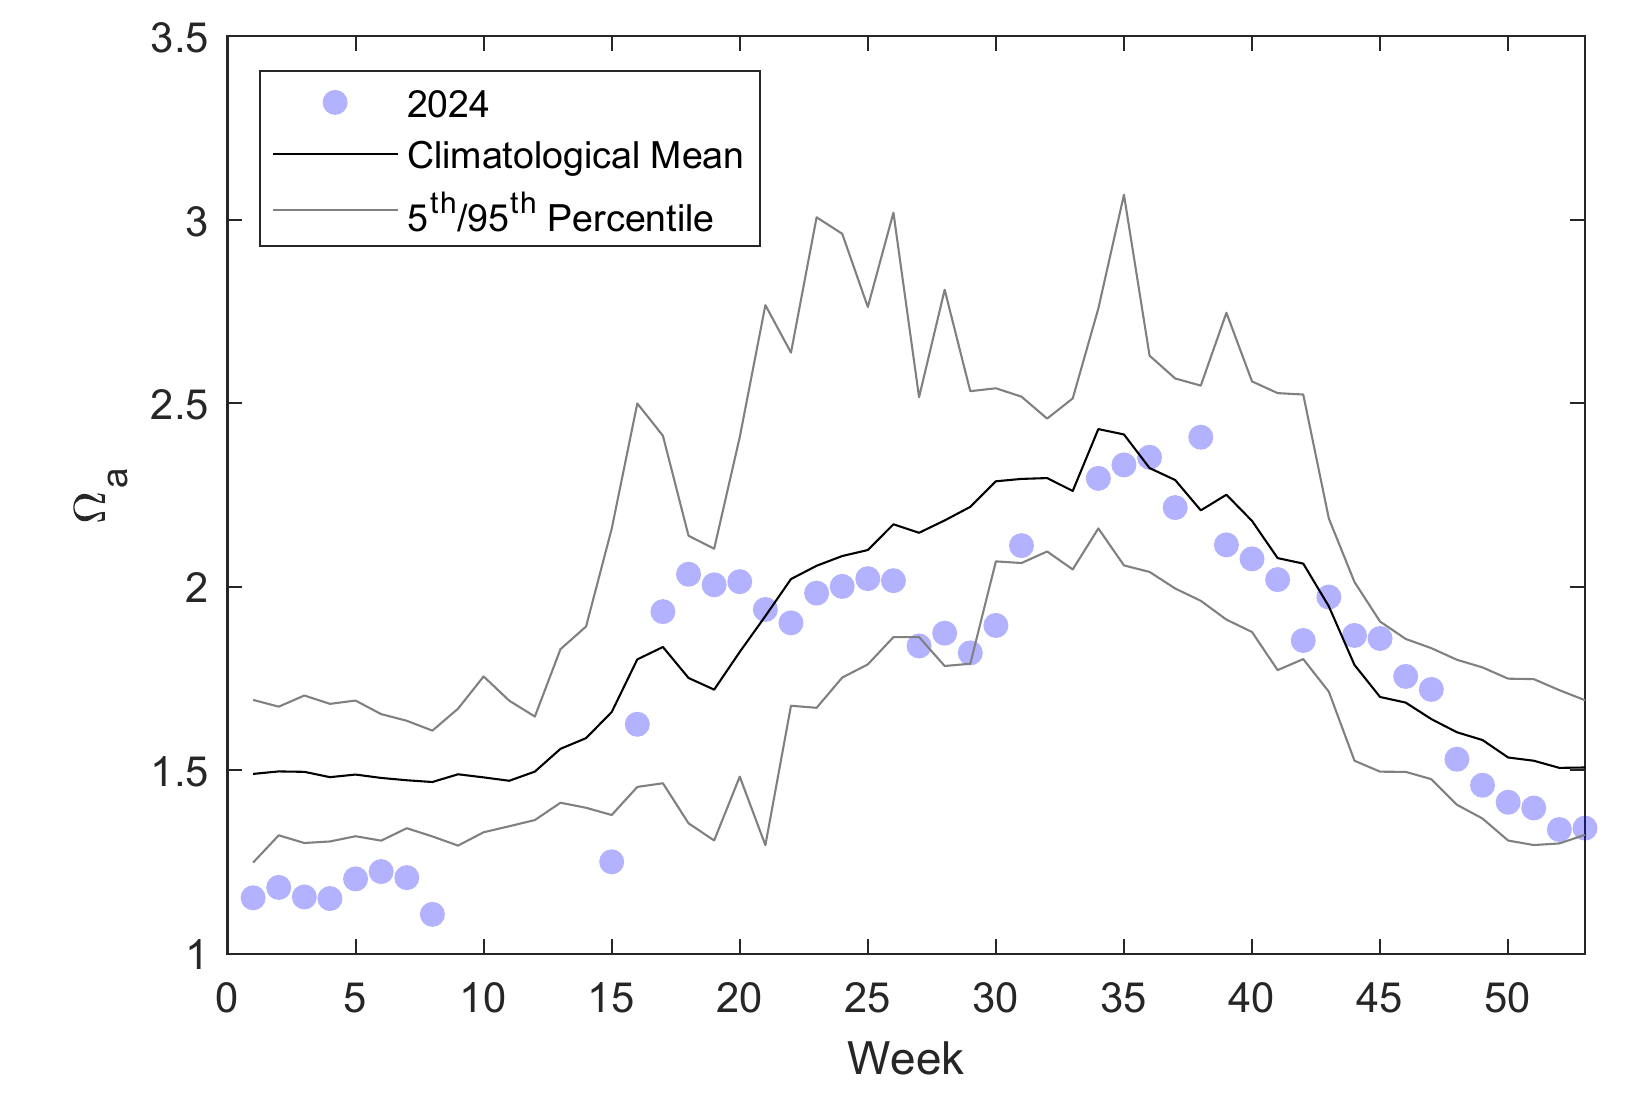
\includegraphics[width=0.6\linewidth]{midatlantic_files/figure-latex/GOMoa-1} 

}

\caption{Weekly average surface aragonite saturation state measured at the long-term buoy location in the Gulf of Maine at 43.02 N and 70.54 W}\label{fig:GOMoa}
\end{figure}

In contrast to the documented die-off of scallops in the Mid-Atlantic Elephant Trunk region between the 2022 and 2023 surveys, in 2024 there was strong scallop recruitment in the southeastern portion of the Nantucket Lightship Area.

\section{Contributors}\label{contributors}

\textbf{Editors} (NOAA NMFS Northeast Fisheries Science Center, NEFSC): Sarah Gaichas, Joseph Caracappa, Andy Beet, Brandon Beltz, Geret DePiper, Kimberly Hyde, Scott Large, Sarah Weisberg.

\textbf{Contributors} (NEFSC unless otherwise noted): Andrew Applegate (NEFMC), Kimberly Bastille, Aaron Beaver (Anchor QEA), Andy Beet, Brandon Beltz, Ruth Boettcher (Virginia Department of Game and Inland Fisheries), Mandy Bromilow (NOAA Chesapeake Bay Office), Joseph Caracappa, Samuel Chavez-Rosales, Baoshan Chen (Stony Brook University), Zhuomin Chen (UConn), Doug Christel (GARFO), Patricia Clay, Lisa Colburn, Jennifer Cudney (NMFS Atlantic HMS Management Division), Tobey Curtis (NMFS Atlantic HMS Management Division), Art Degaetano (Cornell U), Geret DePiper, Bart DiFiore (GMRI), Emily Farr (NMFS Office of Habitat Conservation), Michael Fogarty, Paula Fratantoni, Kevin Friedland, Marjy Friedrichs (VIMS), Sarah Gaichas, Ben Galuardi (GAFRO), Avijit Gangopadhyay (School for Marine Science and Technology, University of Massachusetts Dartmouth), James Gartland (VIMS), Lori Garzio (Rutgers University), Glen Gawarkiewicz (WHOI), Laura Gruenburg, Sean Hardison, Dvora Hart, Cliff Hutt (NMFS Atlantic HMS Management Division), Kimberly Hyde, John Kocik, Steve Kress (National Audubon Society's Seabird Restoration Program), Young-Oh Kwon (Woods Hole Oceanographic Institution), Scott Large, Gabe Larouche (Cornell U), Daniel Linden, Andrew Lipsky, Sean Lucey (RWE), Don Lyons (National Audubon Society's Seabird Restoration Program), Chris Melrose, Anna Mercer, Shannon Meseck, Ryan Morse, Ray Mroch (SEFSC), Brandon Muffley (MAFMC), Robert Murphy, Kimberly Murray, NEFSC staff, David Moe Nelson (NCCOS), Chris Orphanides, Richard Pace, Debi Palka, Tom Parham (Maryland DNR), CJ Pellerin (NOAA Chesapeake Bay Office), Charles Perretti, Kristin Precoda, Grace Roskar (NMFS Office of Habitat Conservation), Jeffrey Runge (U Maine), Grace Saba (Rutgers University), Vincent Saba, Sarah Salois, Chris Schillaci (GARFO), Amy Schueller (SEFSC), Teresa Schwemmer (URI), Tarsila Seara, Dave Secor (CBL), Emily Slesinger, Angela Silva, Adrienne Silver (UMass/SMAST), Talya tenBrink (GARFO), Abigail Tyrell, Rebecca Van Hoeck, Bruce Vogt (NOAA Chesapeake Bay Office), Ron Vogel (University of Maryland Cooperative Institute for Satellite Earth System Studies and NOAA/NESDIS Center for Satellite Applications and Research), John Walden, Harvey Walsh, Sarah Weisberg, Changhua Weng, Dave Wilcox (VIMS), Timothy White (Environmental Studies Program, BOEM), Sarah Wilkin (NMFS Office of Protected Resources), Mark Wuenschel, Qian Zhang (U Maryland).

\section{Document Orientation}\label{document-orientation}

The figure format is illustrated in Fig \ref{fig:docformat}a. Trend lines are shown when slope is significantly different from 0 at the p \textless{} 0.05 level. An orange line signifies an overall positive trend, and purple signifies a negative trend. To minimize bias introduced by small sample size, no trend is fit for \textless{} 30 year time series. Dashed lines represent mean values of time series unless the indicator is an anomaly, in which case the dashed line is equal to 0. Shaded regions indicate the past ten years. If there are no new data for 2022, the shaded region will still cover this time period. The spatial scale of indicators is either coastwide, Mid-Atlantic states (New York, New Jersey, Delaware, Maryland, Virginia, North Carolina), or at the Mid-Atlantic Bight (MAB) Ecosystem Production Unit (EPU, Fig. \ref{fig:docformat}b) level.

\begin{figure}

{\centering 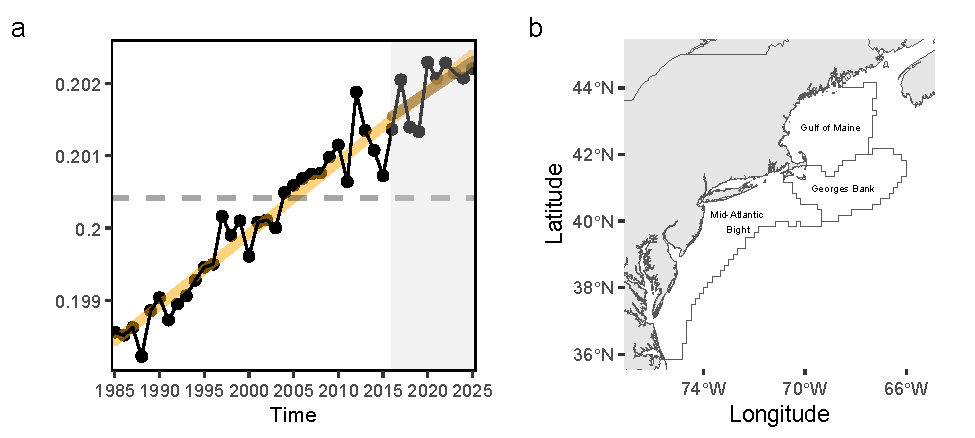
\includegraphics{C:/Users/abigail.tyrell/Documents/code/READ-EDAB-SOE_reports/midatlantic_files/figure-latex/docformat-1} 

}

\caption{Document orientation. a. Key to figures. b.The Northeast Large Marine Ecosystem.}\label{fig:docformat}
\end{figure}

Fish and invertebrates are aggregated into similar feeding categories (Table \ref{tab:species-groupings}) to evaluate ecosystem level trends in predators and prey.

\global\setlength{\Oldarrayrulewidth}{\arrayrulewidth}

\global\setlength{\Oldtabcolsep}{\tabcolsep}

\setlength{\tabcolsep}{2pt}

\renewcommand*{\arraystretch}{1.5}



\providecommand{\ascline}[3]{\noalign{\global\arrayrulewidth #1}\arrayrulecolor[HTML]{#2}\cline{#3}}

\begin{longtable}[c]{|p{1.00in}|p{1.00in}|p{1.00in}|p{1.00in}|p{3.00in}}

\caption{Feeding\ guilds\ and\ management\ bodies.}\label{tab:species-groupings}\\

\ascline{1.5pt}{666666}{1-5}

\multicolumn{1}{>{\raggedright}m{\dimexpr 1in+0\tabcolsep}}{\textcolor[HTML]{000000}{\fontsize{8}{8}\selectfont{Guild}}} & \multicolumn{1}{>{\raggedright}m{\dimexpr 1in+0\tabcolsep}}{\textcolor[HTML]{000000}{\fontsize{8}{8}\selectfont{MAFMC}}} & \multicolumn{1}{>{\raggedright}m{\dimexpr 1in+0\tabcolsep}}{\textcolor[HTML]{000000}{\fontsize{8}{8}\selectfont{Joint}}} & \multicolumn{1}{>{\raggedright}m{\dimexpr 1in+0\tabcolsep}}{\textcolor[HTML]{000000}{\fontsize{8}{8}\selectfont{NEFMC}}} & \multicolumn{1}{>{\raggedright}m{\dimexpr 3in+0\tabcolsep}}{\textcolor[HTML]{000000}{\fontsize{8}{8}\selectfont{State\ or\ Other}}} \\

\ascline{1.5pt}{666666}{1-5}\endfirsthead \caption[]{Feeding\ guilds\ and\ management\ bodies.}\label{tab:species-groupings}\\

\ascline{1.5pt}{666666}{1-5}

\multicolumn{1}{>{\raggedright}m{\dimexpr 1in+0\tabcolsep}}{\textcolor[HTML]{000000}{\fontsize{8}{8}\selectfont{Guild}}} & \multicolumn{1}{>{\raggedright}m{\dimexpr 1in+0\tabcolsep}}{\textcolor[HTML]{000000}{\fontsize{8}{8}\selectfont{MAFMC}}} & \multicolumn{1}{>{\raggedright}m{\dimexpr 1in+0\tabcolsep}}{\textcolor[HTML]{000000}{\fontsize{8}{8}\selectfont{Joint}}} & \multicolumn{1}{>{\raggedright}m{\dimexpr 1in+0\tabcolsep}}{\textcolor[HTML]{000000}{\fontsize{8}{8}\selectfont{NEFMC}}} & \multicolumn{1}{>{\raggedright}m{\dimexpr 3in+0\tabcolsep}}{\textcolor[HTML]{000000}{\fontsize{8}{8}\selectfont{State\ or\ Other}}} \\

\ascline{1.5pt}{666666}{1-5}\endhead



\multicolumn{1}{>{\raggedright}m{\dimexpr 1in+0\tabcolsep}}{\textcolor[HTML]{000000}{\fontsize{8}{8}\selectfont{Apex\ Predator}}} & \multicolumn{1}{>{\raggedright}m{\dimexpr 1in+0\tabcolsep}}{\textcolor[HTML]{000000}{\fontsize{8}{8}\selectfont{}}} & \multicolumn{1}{>{\raggedright}m{\dimexpr 1in+0\tabcolsep}}{\textcolor[HTML]{000000}{\fontsize{8}{8}\selectfont{}}} & \multicolumn{1}{>{\raggedright}m{\dimexpr 1in+0\tabcolsep}}{\textcolor[HTML]{000000}{\fontsize{8}{8}\selectfont{}}} & \multicolumn{1}{>{\raggedright}m{\dimexpr 3in+0\tabcolsep}}{\textcolor[HTML]{000000}{\fontsize{8}{8}\selectfont{shark\ uncl,\ swordfish,\ yellowfin\ tuna,\ bluefin\ tuna}}} \\





\multicolumn{1}{>{\raggedright}m{\dimexpr 1in+0\tabcolsep}}{\textcolor[HTML]{000000}{\fontsize{8}{8}\selectfont{Piscivore}}} & \multicolumn{1}{>{\raggedright}m{\dimexpr 1in+0\tabcolsep}}{\textcolor[HTML]{000000}{\fontsize{8}{8}\selectfont{summer\ flounder,\ bluefish,\ northern\ shortfin\ squid,\ longfin\ squid}}} & \multicolumn{1}{>{\raggedright}m{\dimexpr 1in+0\tabcolsep}}{\textcolor[HTML]{000000}{\fontsize{8}{8}\selectfont{spiny\ dogfish,\ goosefish}}} & \multicolumn{1}{>{\raggedright}m{\dimexpr 1in+0\tabcolsep}}{\textcolor[HTML]{000000}{\fontsize{8}{8}\selectfont{winter\ skate,\ clearnose\ skate,\ thorny\ skate,\ offshore\ hake,\ silver\ hake,\ atlantic\ cod,\ pollock,\ white\ hake,\ red\ hake,\ atlantic\ halibut,\ acadian\ redfish}}} & \multicolumn{1}{>{\raggedright}m{\dimexpr 3in+0\tabcolsep}}{\textcolor[HTML]{000000}{\fontsize{8}{8}\selectfont{sea\ lamprey,\ sandbar\ shark,\ atlantic\ angel\ shark,\ atlantic\ torpedo,\ conger\ eel,\ spotted\ hake,\ cusk,\ fourspot\ flounder,\ windowpane,\ john\ dory,\ atlantic\ cutlassfish,\ blue\ runner,\ striped\ bass,\ weakfish,\ sea\ raven,\ northern\ stargazer,\ banded\ rudderfish,\ atlantic\ sharpnose\ shark,\ inshore\ lizardfish,\ atlantic\ brief\ squid,\ northern\ sennet,\ king\ mackerel,\ spanish\ mackerel}}} \\





\multicolumn{1}{>{\raggedright}m{\dimexpr 1in+0\tabcolsep}}{\textcolor[HTML]{000000}{\fontsize{8}{8}\selectfont{Planktivore}}} & \multicolumn{1}{>{\raggedright}m{\dimexpr 1in+0\tabcolsep}}{\textcolor[HTML]{000000}{\fontsize{8}{8}\selectfont{atlantic\ mackerel,\ chub\ mackerel,\ butterfish}}} & \multicolumn{1}{>{\raggedright}m{\dimexpr 1in+0\tabcolsep}}{\textcolor[HTML]{000000}{\fontsize{8}{8}\selectfont{}}} & \multicolumn{1}{>{\raggedright}m{\dimexpr 1in+0\tabcolsep}}{\textcolor[HTML]{000000}{\fontsize{8}{8}\selectfont{atlantic\ herring}}} & \multicolumn{1}{>{\raggedright}m{\dimexpr 3in+0\tabcolsep}}{\textcolor[HTML]{000000}{\fontsize{8}{8}\selectfont{harvestfishes,\ smelts,\ round\ herring,\ alewife,\ blueback\ herring,\ american\ shad,\ menhaden,\ bay\ anchovy,\ striped\ anchovy,\ rainbow\ smelt,\ atlantic\ argentine,\ slender\ snipe\ eel,\ atlantic\ silverside,\ northern\ pipefish,\ atlantic\ moonfish,\ lookdown,\ blackbelly\ rosefish,\ lumpfish,\ northern\ sand\ lance,\ atlantic\ saury,\ mackerel\ scad,\ bigeye\ scad,\ round\ scad,\ rough\ scad,\ silver\ rag,\ weitzmans\ pearlsides,\ atlantic\ soft\ pout,\ sevenspine\ bay\ shrimp,\ pink\ glass\ shrimp,\ polar\ lebbeid,\ friendly\ blade\ shrimp,\ bristled\ longbeak,\ aesop\ shrimp,\ norwegian\ shrimp,\ northern\ shrimp,\ brown\ rock\ shrimp,\ atlantic\ thread\ herring,\ spanish\ sardine,\ atlantic\ bumper,\ harvestfish,\ striated\ argentine,\ silver\ anchovy}}} \\





\multicolumn{1}{>{\raggedright}m{\dimexpr 1in+0\tabcolsep}}{\textcolor[HTML]{000000}{\fontsize{8}{8}\selectfont{Benthivore}}} & \multicolumn{1}{>{\raggedright}m{\dimexpr 1in+0\tabcolsep}}{\textcolor[HTML]{000000}{\fontsize{8}{8}\selectfont{black\ sea\ bass,\ scup,\ tilefish}}} & \multicolumn{1}{>{\raggedright}m{\dimexpr 1in+0\tabcolsep}}{\textcolor[HTML]{000000}{\fontsize{8}{8}\selectfont{}}} & \multicolumn{1}{>{\raggedright}m{\dimexpr 1in+0\tabcolsep}}{\textcolor[HTML]{000000}{\fontsize{8}{8}\selectfont{barndoor\ skate,\ rosette\ skate,\ little\ skate,\ smooth\ skate,\ haddock,\ american\ plaice,\ yellowtail\ flounder,\ winter\ flounder,\ witch\ flounder,\ atlantic\ wolffish,\ ocean\ pout,\ crab,red\ deepsea}}} & \multicolumn{1}{>{\raggedright}m{\dimexpr 3in+0\tabcolsep}}{\textcolor[HTML]{000000}{\fontsize{8}{8}\selectfont{crab,unc,\ hagfish,\ porgy,red,\ sea\ bass,nk,\ atlantic\ hagfish,\ roughtail\ stingray,\ smooth\ dogfish,\ chain\ dogfish,\ bluntnose\ stingray,\ bullnose\ ray,\ southern\ stingray,\ longfin\ hake,\ fourbeard\ rockling,\ marlin-spike,\ gulf\ stream\ flounder,\ longspine\ snipefish,\ blackmouth\ bass,\ threespine\ stickleback,\ smallmouth\ flounder,\ hogchoker,\ bigeye,\ atlantic\ croaker,\ pigfish,\ northern\ kingfish,\ silver\ perch,\ spot,\ deepbody\ boarfish,\ sculpin\ uncl,\ moustache\ sculpin,\ longhorn\ sculpin,\ alligatorfish,\ grubby,\ atlantic\ seasnail,\ northern\ searobin,\ striped\ searobin,\ armored\ searobin,\ cunner,\ tautog,\ snakeblenny,\ daubed\ shanny,\ radiated\ shanny,\ red\ goatfish,\ striped\ cusk-eel,\ wolf\ eelpout,\ wrymouth,\ fawn\ cusk-eel,\ northern\ puffer,\ striped\ burrfish,\ planehead\ filefish,\ gray\ triggerfish,\ shortnose\ greeneye,\ beardfish,\ cownose\ ray,\ american\ lobster,\ cancer\ crab\ uncl,\ jonah\ crab,\ atlantic\ rock\ crab,\ blue\ crab,\ spider\ crab\ uncl,\ horseshoe\ crab,\ coarsehand\ lady\ crab,\ lady\ crab,\ northern\ stone\ crab,\ snow\ crab,\ spiny\ butterfly\ ray,\ smooth\ butterfly\ ray,\ snakefish,\ atlantic\ midshipman,\ bank\ cusk-eel,\ red\ cornetfish,\ squid\ cuttlefish\ and\ octopod\ uncl,\ spoonarm\ octopus,\ bank\ sea\ bass,\ rock\ sea\ bass,\ sand\ perch,\ cobia,\ crevalle\ jack,\ vermilion\ snapper,\ tomtate,\ jolthead\ porgy,\ saucereye\ porgy,\ whitebone\ porgy,\ knobbed\ porgy,\ sheepshead\ porgy,\ littlehead\ porgy,\ silver\ porgy,\ pinfish,\ red\ porgy,\ porgy\ and\ pinfish\ uncl,\ banded\ drum,\ southern\ kingfish,\ atlantic\ spadefish,\ leopard\ searobin,\ dusky\ flounder,\ triggerfish\ filefish\ uncl,\ blackcheek\ tonguefish,\ orange\ filefish,\ queen\ triggerfish,\ ocean\ triggerfish}}} \\





\multicolumn{1}{>{\raggedright}m{\dimexpr 1in+0\tabcolsep}}{\textcolor[HTML]{000000}{\fontsize{8}{8}\selectfont{Benthos}}} & \multicolumn{1}{>{\raggedright}m{\dimexpr 1in+0\tabcolsep}}{\textcolor[HTML]{000000}{\fontsize{8}{8}\selectfont{atlantic\ surfclam,\ ocean\ quahog}}} & \multicolumn{1}{>{\raggedright}m{\dimexpr 1in+0\tabcolsep}}{\textcolor[HTML]{000000}{\fontsize{8}{8}\selectfont{}}} & \multicolumn{1}{>{\raggedright}m{\dimexpr 1in+0\tabcolsep}}{\textcolor[HTML]{000000}{\fontsize{8}{8}\selectfont{sea\ scallop}}} & \multicolumn{1}{>{\raggedright}m{\dimexpr 3in+0\tabcolsep}}{\textcolor[HTML]{000000}{\fontsize{8}{8}\selectfont{sea\ cucumber,\ sea\ urchins,\ snails(conchs),\ sea\ urchin\ and\ sand\ dollar\ uncl,\ channeled\ whelk,\ blue\ mussel}}} \\

\ascline{1.5pt}{666666}{1-5}



\end{longtable}



\arrayrulecolor[HTML]{000000}

\global\setlength{\arrayrulewidth}{\Oldarrayrulewidth}

\global\setlength{\tabcolsep}{\Oldtabcolsep}

\renewcommand*{\arraystretch}{1}

\end{document}
